%% Template para dissertação/tese na classe UFPEthesis
%% versão 0.9.2
%% (c) 2005 Paulo G. S. Fonseca
%% www.cin.ufpe.br/~paguso/ufpethesis

%% Carrega a classe ufpethesis
%% Opções: * Idiomas
%%           pt   - português (padrão)
%%           en   - inglês
%%         * Tipo do Texto
%%           bsc  - para monografias de graduação
%%           msc  - para dissertações de mestrado (padrão)
%%           qual - exame de qualificação doutorado
%%           prop - proposta de tese doutorado
%%           phd  - para teses de doutorado
%%         * Mídia
%%           scr  - para versão eletrônica (PDF) / consulte o guia do usuario
%%         * Estilo
%%           classic - estilo original à la TAOCP (deprecated)
%%           std     - novo estilo à la CUP (padrão)
%%         * Paginação
%%           oneside - para impressão em face única
%%           twoside - para impressão em frente e verso (padrão)
\documentclass[bsc, oneside]{UFPEThesis/ufpethesis}

%% Preâmbulo:
%% coloque aqui o seu preâmbulo LaTeX, i.e., declaração de pacotes,
%% (re)definições de macros, medidas, etc.

%% Identificação:

% Universidade
% e.g. \university{Universidade de Campinas}
% Na UFPE, comente a linha a seguir
\university{Universidade Federal de Pernambuco}

% Endereço (cidade)
% e.g. \address{Campinas}
% Na UFPE, comente a linha a seguir
% \address{<CIDADE DA IES>}

% Instituto ou Centro Acadêmico
% e.g. \institute{Centro de Ciências Exatas e da Natureza}
% Comente se não se aplicar
\institute{Centro de Informática}

% Departamento acadêmico
% e.g. \department{Departamento de Informática}
% Comente se não se aplicar
% \department{<NOME DO DEPARTAMENTO>}

% Programa de pós-graduação
% e.g. \program{Pós-graduação em Ciência da Computação}
\program{Bacharelado em Ciência da Computação}

% Área de titulação
% e.g. \majorfield{Ciência da Computação}
\majorfield{Ciência da Computação}

% Título da dissertação/tese
% e.g. \title{Sobre a conjectura $P=NP$}
\title{Previsão imediata de sequências de sinais de áudio como método de redução de latência em transmissões online}

% Data da defesa
% e.g. \date{19 de fevereiro de 2003}
% \date{<DATA DA DEFESA>}

% Autor
% e.g. \author{José da Silva}
\author{Luiz Henrique Tavares Caúla}

% Orientador(a)
% Opção: [f] - para orientador do sexo feminino
% e.g. \adviser[f]{Profa. Dra. Maria Santos}
\adviser{Filipe Carlos de Albuquerque Calegario}

% Orientador(a)
% Opção: [f] - para orientador do sexo feminino
% e.g. \coadviser{Prof. Dr. Pedro Pedreira}
% Comente se não se aplicar
% \coadviser{NOME DO(DA) CO-ORIENTADOR(A)}

%% Inicio do documento
\begin{document}

%%
%% Parte pré-textual
%%
\frontmatter

% Folha de rosto
% Comente para ocultar
\frontpage

% Portada (apresentação)
% Comente para ocultar
\presentationpage

% Dedicatória
% Comente para ocultar
% \begin{dedicatory}
% <DIGITE A DEDICATÒRIA AQUI>
% \end{dedicatory}

% Agradecimentos
% Se preferir, crie um arquivo à parte e o inclua via \include{}
\acknowledgements

TODO: Agradecimentos

% Epígrafe
% Comente para ocultar
% e.g.
%  \begin{epigraph}[Tarde, 1919]{Olavo Bilac}
%  Última flor do Lácio, inculta e bela,\\
%  És, a um tempo, esplendor e sepultura;\\
%  Ouro nativo, que, na ganga impura,\\
%  A bruta mina entre os cascalhos vela.
%  \end{epigraph}
% \begin{epigraph}[<NOTA>]{<AUTOR>}
% <DIGITE AQUI A CITAÇÂO>
% \end{epigraph}

% Resumo em Português
% Se preferir, crie um arquivo à parte e o inclua via \include{}
\resumo
\addcontentsline{toc}{chapter}{Resumo}

Devido à alta sensibilidade do aparelho auditivo humano, para performar em conjunto com outros artistas, músicos necessitam que haja pouca latência entre a saída dos instrumentos de seus colegas e seu retorno. Dessa forma, proporcionar um ambiente colaborativo em tempo real via Internet torna-se um desafio pertinente na área de Computação Musical e Rede de Computadores. Algumas soluções procuram otimizar a conexão entre os computadores construindo infraestruturas dedicadas ou abandonam o requisito de tempo real ao entregar experiências assíncronas. No entanto, tais abordagens não abrangem, de forma síncrona, casos em que não haja acesso a uma conexão de alta velocidade ou que exista uma grande distância entre os participantes.

Este trabalho propõe, dessa forma, uma adaptação do algoritmo \textit{Client-Side Prediction}, utilizado em \textit{videogames online}, experimentando dois modelos preditivos para gerar novas sequências de áudio baseando-se nas anteriores - predição de sequências com LSTM (\textit{Long Short-Term Memory}) e indexação e identificação de sequências com DTW (\textit{Dynamic Time Warping}). De tal forma, espera-se que, não sendo necessária a espera pela saída do cliente transmissor, haja uma redução da percepção de latência por parte dos participantes.

Utilizando duas métricas de sucesso - corretude das previsões e tempo de processamento - avaliamos que o modelo gerador com LSTM não performou bem comparado ao modelo indexador com DTW, que apresentou resultados bastante promissores e que pode ser utilizado para músicas de gêneros com tendências menos improvisacionais.

\begin{keywords}
latência, áudio, predição de sequência, streaming, transmissão, online, música, client-side prediction, rollback, dtw, lstm
\end{keywords}


% Resumo em Inglês
% Se preferir, crie um arquivo à parte e o inclua via \include{}
% \abstract
% Palavras-chave do resumo em Inglês
% \begin{keywords}
% <DIGITE AS PALAVRAS-CHAVE AQUI>
% \end{keywords}

% Sumário
% Comente para ocultar
\tableofcontents

% Lista de figuras
% Comente para ocultar
\listoffigures

% Lista de tabelas
% Comente para ocultar
\listoftables



%%
%% Parte textual
%%
\mainmatter

% É aconselhável criar cada capítulo em um arquivo à parte, digamos
% "capitulo1.tex", "capitulo2.tex", ... "capituloN.tex" e depois
% incluí-los com:
\chapter{Introdução}

A performance artística musical, quando praticada em conjunto, requer alto nível de colaboração entre os participantes. Em música, sobretudo gêneros com tendências improvisacionais como \textit{jazz}, \textit{blues} e \textit{rock}, o ato de ouvir e reagir ao som de seus companheiros é tão importante quanto aquele produzido individualmente. Dessa forma, o \textit{feedback} auditivo de baixa latência dos instrumentos tocados é fundamental para que haja uma sensação fluida entre os participantes.

Normalmente, músicos performando em conjunto em um mesmo ambiente físico raramente experienciarão problemas relacionados à latência. No entanto, em um contexto de distanciamento social, encorajado durante à Pandemia de COVID-19 no ano de 2020, músicos ao redor do mundo viram-se obrigados a transferirem esse ambiente para um virtual \textit{online}.

% Devido à abordagem de "melhor esforço" em que a Internet foi originalmente projetada - sob a suposição de que não é possível garantir o recebimento de todos os pacotes transmitidos - protocolos de transmissão de voz como \textit{VoIP} (\textit{Voice over Internet Protocol}) e serviços provedores videoconferências necessitam implementar medidas compensatórias, como grandes \textit{buffers} de rede e retransmissão de pacotes. Tais medidas, consequentemente, garantem a corretude dos dados transmitidos, sob o custo do aumento na latência total \cite{carot_low_latency}. Para aplicações comuns, essa troca é aceitável; entretanto, no contexto da arte musical colaborativa, mostra-se inviável.

Aplicações comerciais de videoconferências, como o \textit{Zoom}, \textit{Google Meet} e \textit{FaceTime}  possuem sensibilidade de tempo para manter conversas compreensíveis - a \textit{Cisco} define a latência máxima aceitável de uma implementação \textit{VoIP} em até 150 ms \cite{cisco}. Este limite, apesar de relativamente baixo, pode ser alcançado por conexões de velocidades medianas, implementações de processamento de áudio e infraestruturas de rede compartilhadas. No entanto, para a prática colaborativa musical, onde tolerância máxima é bastante restrita - variando entre 10 ms e 55 ms \cite{mcphearson} - mostra-se inviável. Em ambientes de alta latência, músicos tendem a perceber incômodos e mudam a forma sobre como performam para adptarem-se. \cite{carot_low_latency}.

Para lidar com estes problemas, \textit{softwares} voltados especificamente para a colaboração musical \textit{online} apresentam uma variedade de abordagens diferentes. \textit{LoLa} \cite{lola}, \textit{SoundJack} \cite{soundjack} e \textit{JamKazam} \cite{jamkazam}, por exemplo, implementam otimizações na camada de rede - como conectar clientes diretamente entre si via \textit{P2P} (\textit{peer-to-peer}) - oferecendo latências aceitáveis entre distâncias medianas. Outras aplicações, como o \textit{Jammr} \cite{jammr}, dispensam o requisito de tempo real e apresentam soluções assíncronas, onde os músicos ouvem os últimos quatro compassos tocados por seus companheiros em um \textit{loop} contínuo.

No entanto, tais abordagens não abrangem casos onde não é possível ter acesso a conexões dedicadas ou os músicos residem entre grandes distâncias, ainda mantendo uma performance síncrona.

Ao observar o contexto de videogames, encontramos requisitos de latência similares. Gêneros que utilizam reações como mecânica de jogabilidade, como luta e FPS (\textit{first-person shooter}), para oferecerem aos jogadores uma experiência fluida, necessitam de latências máximas de até 100 ms \cite{pubnub}. O algoritmo mais popular e efetivo para solucionar esse problema, \textit{Rollback Netcode} \cite{rollback}, baseia-se em prever os próximos \textit{inputs} imediatos dos jogadores e agindo antes mesmo que os dados de seu oponente sejam transmitidos; desta forma, removendo qualquer necessidade de espera. Uma vez que os \textit{inputs} são recebidos, estes são comparados com a previsão realizada e, caso sejam incongruentes entre si, o jogo é retornado ao estado anterior do momento da previsão inicial.

Por possuir contextos semelhantes, a mesma implementação baseada em previsões tem o potencial de resolver o problema descrito anteriormente para ambientes musicais colaborativos \textit{online}. Caso seja possível prever os próximos sinais digitais produzidos pelos artistas remotos, não haveria necessidade de espera e, portanto, a latência de rede tornaria-se irrelevante. É  evidente que, entretanto, por apresentar uma linearidade no tempo, não é possível retornar ao último momento da música anterior à previsão imediata. Portanto, é necessário que o modelo preditivo seja o mais acurado possível, visando minimizar a quantidade total de erros.

\chapter{Contexto}

Neste Capítulo, descreveremos em maiores detalhes o problema da latência no contexto de aplicações musicais colaborativas \textit{online}, além de explorar soluções que procuram resolvê-lo. Por último, demonstraremos a inspiração da solução proposta, o \textit{Rollback Netcode}, dentro do contexto de videogames, como ele se relaciona com o problema original e como propomos aplicá-lo no ambiente musical.

\section{O problema}

% Qual o problema que vai ser tratado? Por que ele é complexo? Por que ele é relevante?
% O que se espera de uma solução para o problema? quais são os critérios de avaliação
% de uma solução? escalabilidade, corretude, facilidade de uso, etc.?

A execução musical praticada em conjunto é altamente colaborativa. Em gêneros com tendências improvisacionais, como \textit{jazz}, \textit{blues} e \textit{rock}, é comum que hajam um ou mais integrantes que usam como base os ritmos e conjunto de acordes praticados por seus colegas para executar \textit{solos} que reagem de acordo com as mudanças da harmonia. É importante, portanto, que haja um \textit{feedback} fluído entre o improvisador e a base musical para que todos possuam conhecimento se o que está sendo tocado está de acordo com suas intenções.

Em gêneros mais metódicos, como música clássica, onde os músicos seguem precisamente as instruções de partituras e um condutor, reação à mudanças é menos importante. Porém, ainda é necessária a garantia que todos estejam tocando em sincronia uns com os outros. Para o condutor, é importante que possua ciência do que está sendo executado por cada conjunto de instrumentos, de forma a garantir totalmente a harmonia entre as partes.

Quando performado em conjunto no mesmo ambiente físico, normalmente não há percepção de latência entre os integrantes. Tal latência é baseada na velocidade em que o som se propaga no ar em temperatura ambiente que, em uma velocidade de 343,2 m/s \cite{speed_of_sound}, produz cerca de 3 ms de atraso por metro de distância entre cada músico, sendo negligenciável para a sensação de fluidez dos músicos.

No entanto, em ambientes colaborativos \textit{online}, outros fatores podem interferir na latência total. Primeiramente, para que os computadores do participantes consigam processar o áudio, é necessário que haja uma conversão dos sinais analógicos para digitais. Tal processamento consome cerca de 1 ms \cite{how_low_can_you_go}, podendo ser negligenciada. Uma vez convertidos, os sinais precisam ser escritos e lidos no \textit{buffer} em memória, processo que dura entre 10 ms e 12 ms \cite{how_low_can_you_go}, dependendo do poder de processamento das máquinas envolvidas. Ambos processos ocorrem no lado do transmissor (aquele que produz a música) e dos receptores, portanto, dobrando o tempo total.

O maior gargalo, no entanto, ocorre na transmissão dos pacotes de dados via Internet. Devido à abordagem de "melhor esforço" na qual a Internet foi originalmente projetada - sob a suposição de que não é possível garantir o recebimento de todos os pacotes transmitidos - protocolos de transmissão de voz como \textit{VoIP} (\textit{Voice over Internet Protocol}) e serviços provedores videoconferências necessitam implementar medidas compensatórias, como grandes \textit{buffers} de rede e retransmissão de pacotes. Tais medidas, consequentemente, garantem a corretude dos dados transmitidos, sob o custo do aumento na latência total \cite{carot_low_latency}.

\begin{figure}[htbp]
\centering
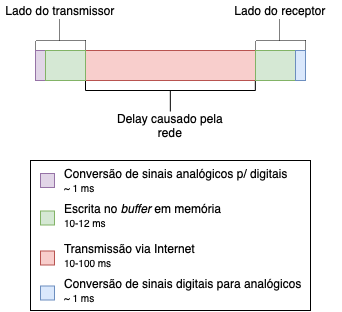
\includegraphics[width=0.5\textwidth]{images/streaming-latency.png}
\caption{Latências de cada fase do processo de \textit{streaming} de áudio pela Internet}
\label{fig:streaming_latencies}
\end{figure}

Aplicações comerciais de videoconferências, como o \textit{Zoom}, \textit{Google Meet} e \textit{FaceTime} também  possuem sensibilidade de tempo para manter conversas compreensíveis - a \textit{Cisco} define a latência máxima aceitável de uma implementação \textit{VoIP} em até 150 ms \cite{cisco}. Este limite pode ser alcançado por conexões de velocidades medianas, mesmo considerando fatores como processamento de áudio, distância entre os participantes e infraestruturas de rede compartilhadas. No entanto, para a prática colaborativa musical, onde tolerância máxima é bastante restrita - variando entre 10 ms e 55 ms \cite{mcphearson} - mostra-se inviável. Em ambientes de alta latência, músicos tendem a perceber incômodos e mudam a forma sobre como performam para adaptarem-se. \cite{carot_low_latency}.

A tolerância de atraso para a performance musical, portanto, é o maior desafio na implementação de ambientes colaborativos musicais \textit{online}. Afinal, mesmo considerando a velocidade da luz no vácuo - aproximadamente 300 km/ms \cite{speed_of_light} - a menor distância possível para obter uma latência ótima de 10 ms é de aproximadamente 3.000 km - um pouco mais que a distância entre Recife, PE e Porto Alegre, RS\footnote{Distância calculada utilizando o Google Maps. ©2021 Google}.

Dessa forma, métodos para redução da latência entre os participantes - ou a sensação de sua existência - possuem suma relevância para músicos. Em contextos onde a presença física dos participantes não é possível de se obter, como o recomendado pelo distanciamento social como método de prevenção de contaminação na Pandemia de COVID-19, a colaboração \textit{online} é o único meio onde músicos conseguem tocar em conjunto.
\section{Estado da arte}

% quais são as soluções atuais para o problema? Como elas atendem os "critérios de avaliaçao"? O que pode serve de inspiração para sua solução?
% no caso de problema/solução original, faz um estado da arte de delimitação do escopo (eu conheo o que existe o suficiente para dizer que ninguém)

Para resolver o problema da latência em ambientes musicais, identificamos duas abordagens principais: (1) otimizações na camada de transporte da Internet e (2) criação de ambientes assíncronos, onde os músicos não performam em tempo real uns com os outros.

\subsection{Otimizações na camada de transporte}

Esta abordagem procura atacar o problema de forma mais linear, implementando melhorias na conexão pela Internet entre os participantes ou utilizando infraestruturas de rede específicas.

\textit{LoLa} (\textit{LOw LAtency audio visual streaming system}) \cite{lola}, um sistema de \textit{streaming} audio visual desenvolvido pelo \textit{Conservatorio di Musica G. Tartini}, consegue atingir conexões de baixa latência, utilizando infraestruturas de rede dedicadas. Foi usado em diversas apresentações de até 3.500 km de distância entre os músicos entre os anos de 2010 e 2013 \cite{lola_streaming}. No entanto, deixa muito claro que sua solução não é necessariamente acessível, sendo recomendado no mínimo 1 Gigabit por segundo de banda em todas as pontas. De acordo com estudo realizado pela Viavi Solutions em 2019, apenas 5\% da população mundial possui conexões tão rápidas \cite{1gbps}, e a média de velocidade mundial é de apenas 97.52 Megabits por segundo, pelos dados apresentados pelo Speedtest Global Index \cite{speed_test}. Portanto, para o público em geral, não é uma solução de fácil acesso.

\textit{SoundJack} \cite{soundjack}, por outro lado, utiliza-se de alguns métodos que o torna mais acessíveis para o usuário comum. Ele consegue atingir velocidades mais rápidas que aplicações comerciais como \textit{Zoom}, \textit{Teams} e \textit{FaceTime} por dois fatores: (1) conecta usuários diretamente através de P2P (\textit{peer-to-peer}), ao contrário das soluções citadas, que transportam dados entre servidores centrais e (2) não otimiza a qualidade o áudio/vídeo automaticamente, deixando como responsabilidade do usuário; caso prefiram, os músicos podem optar por conexões de menores latências assumindo o custo de obter piores qualidades de áudio. Nas configurações recomendadas, infraestruturas comerciais comuns residenciais são suportadas via Ethernet. Entretanto, \textit{SoundJack} requer um poder computacional relativamente alto para atingir baixas latências - recomenda no mínimo processadores i7 Quad Core, custando cerca de R\$2456,90 \footnote{Preço encontrado na Amazon Brasil em 04/04/2021.}, também oferecendo um dispositivo próprio dedicado à aplicação, vendendo por €226,05 \footnote{Preço encontrado na Symonics em 04/04/2021.}.

A aplicação comercial \textit{JamKazam} \cite{jamkazam} também baseia-se em entrega síncrona dos pacotes de áudio para construir um ambiente musical colaborativo \textit{online}. De acordo com seus os resultados apresentados, é possível performar em conjunto com baixas latências onde os músicos estejam em um mesmo estado, numa distância média de 490 km \cite{jamkazam_video}. Porém, entre maiores distâncias ou infraestruturas não baseadas em fibras, a latência excelente recomendada pela aplicação de 30 ms \cite{jamkazam_latencies} é difícil de ser obtida.

TODO: JackTrip

\subsection{Criação de ambientes assíncronos}

Uma solução que possibilita a percepção de baixa latência é abdicar do requisito de entregar uma experiência em tempo real. Caso seja possível atrasar a entrega dos pacotes de forma não perceptível e, portanto, aumentando a janela mínima de espera, não é necessário possuir baixas latências.

A aplicação \textit{jammr} \cite{jammr} aproveita o conceito de progressão de acordes da teoria musical a seu favor. A cada \textit{loop}, os participantes ouvem o que foi tocado na última iteração pelos seus colegas. Dessa forma, por não ser necessário manter as performances em sincronia, há uma tolerância muito maior às latências causadas tanto pela camada de transporte como as causadas pelos processamentos de áudio locais. No entanto, tal solução necessita que os músicos toquem a mesma progressão em \textit{loop}, funcionando bem para improvisações simples (\textit{jam sessions}); porém, para músicas mais complexas, o sistema não é ideal.

\chapter{Ciclo 1: Previsão de sequências com LSTM}

TODO: explicação geral do primeiro ciclo
\section{Proposta de solução}

% • Princípios, inspirações, ideias gerais
% • Descrição detalhada da solução
% • implementação (arquitetura, tecnologias, etc.)

TODO: explicar proposta de solução do LSTM

- Explicar sobre a escolha do tamanho da janela
\section{Avaliação}

% • Metodologia
% • Resultados obtidos
% • Análise: discussão dos resultados

TODO: mostrar resultados.

- Imagem dos sinais sobrepondo-se
- Acabou repetindo os dados de entrada
\chapter{Ciclo 2: Indexação com DTW}

TODO: explicar a ideia do DTW vinda a partir dos resultados do primeiro ciclo
\section{Proposta de solução}

% • Princípios, inspirações, ideias gerais
% • Descrição detalhada da solução
% • implementação (arquitetura, tecnologias, etc.)

TODO: explicar proposta de solução com DTW

- imagem do encontro dos áudios
- relembrar sobre o dilema da escolha de duração da janela
\section{Avaliação}

Para analisar a efetividade desse modelo, vamos analisar sob a ótica os critérios de avaliação, definidos na \secref{sec:success_metrics}.

\subsection{Corretude das previsões}

Para cada um dos valores de $LAG$, definidos na \secref{sec:lstm-metodology}, todas as previsões realizadas tenderam a "repetir" as sequências de áudio de entrada. Comparando os sinais digitais do arquivo de teste e os gerados na previsão, ilustrados na \figref{fig:lstm-repetition-results}, é possível notar que, quando alinhado com a sequência real de teste, não há nenhuma correspondência. No entanto, ao compararmos com os dados de entrada, isto é, o que construímos a lista $Z$, é possível notar uma clara semelhança. O formato da onda sonora foi mantido, diferindo apenas por sua amplitude.

Ademais, os áudios previstos soaram distorcidos, consequência das diferenças de amplitude encontradas nos sinais digitais da previsão contra a sequência de entrada.

Esses resultados foram observados em todas as janelas de entrada, tanto para os valores de $LAG$ 50 ms e 100 ms.

\begin{figure}
     \centering
     \begin{subfigure}[b]{0.49\textwidth}
         \centering
         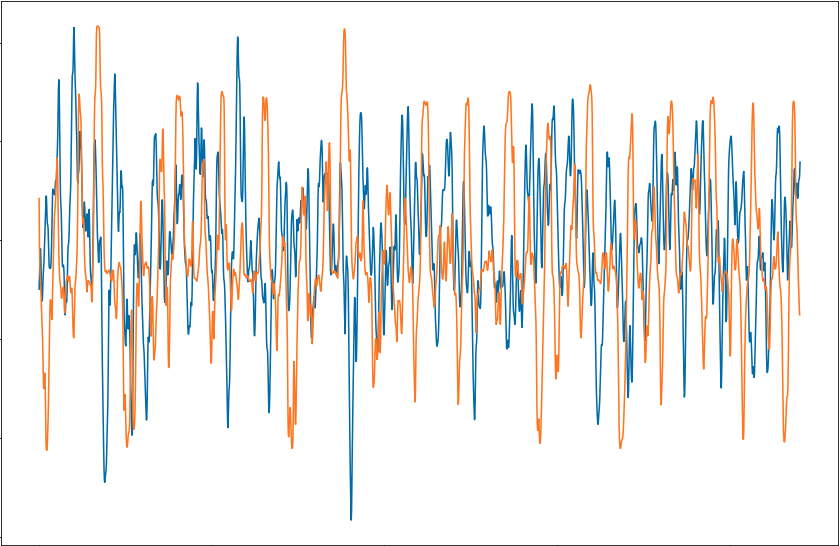
\includegraphics[width=\textwidth]{images/lstm-after.png}
         \caption{Previsão alinhada com a sequência real de teste.}
         \label{fig:y equals x}
     \end{subfigure}
     \hfill
     \begin{subfigure}[b]{0.49\textwidth}
         \centering
         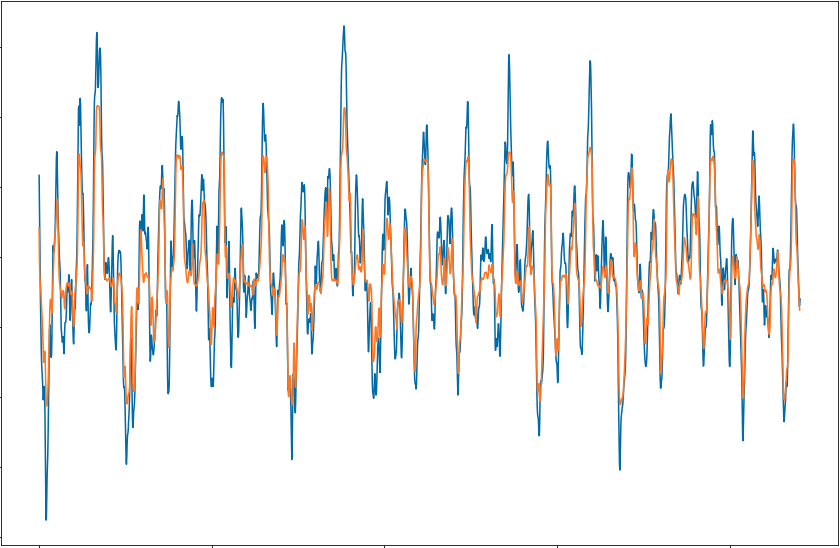
\includegraphics[width=\textwidth]{images/lstm-before.png}
         \caption{Previsão alinhada com a sequência de entrada.}
         \label{fig:three sin x}
     \end{subfigure}
        \caption{Comparação entre as sequências digitais geradas na previsão de uma das listas $Z$, em laranja, com (a) a sequência real de teste e (b) a sequência de entrada, ambas em azul, para o valor $LAG = 50 ms$.}
        \label{fig:lstm-repetition-results}
\end{figure}

Caso aplicássemos esse modelo em uma aplicação real, efetivamente estaríamos repetindo os dados transmitidos e, como discutido no \chapref{chap:solution_propositon}, retornaremos ao problema que as soluções \textit{delay-based} enfrentam. Portanto, não podemos atestar a corretude das previsões para o modelo preditivo gerador de novas sequências.

\subsection{Tempo de geração de previsões}

Na \tabref{tab:lstm-time-results}, podemos observar as médias de tempo para gerar as previsões para cada valor de $LAG$ testado, assim com o tempo médio de treinamento. É notável que, para nenhum dos dois valores, o tempo de previsão foi menor que o tempo da janela de previsão. Dessa forma, podemos afirmar que este modelo preditivo, como foi implementado, não satisfaz a métrica de sucesso para o tempo de previsão.

Ademais, vale notar que, apesar de não ser uma métrica de sucesso, que o tempo médio de treinamento foi relativamente alto, além de depender do valor de $LAG$.

\begin{table}[ht!]
    \centering
    \begin{tabular}{|c||c|c|}
        \hline
        
        Valor de LAG & Média de tempo de previsão & Média de tempo de treinamento por epoch \\
        
        \hline
        \hline
        
        50 ms & 150 ms & 55 s  \\ 
        \hline
        
        100 ms & 380 ms & 127 s \\ 
        \hline
    \end{tabular}
    \caption{Tabela comparando os tempos médios para gerar as previsões e para treinar os modelos para os valores 50 ms e 100 ms de simulação de latência da Internet.}
    \label{tab:lstm-time-results}
\end{table}

\chapter{Conclusões}

% • Contribuições: o que voce trouxe de novo?
% • trabalhos futuros

%%
%% Parte pós-textual
%%
\backmatter

% Apêndices
% Comente se não houver apêndices
\appendix

% É aconselhável criar cada apêndice em um arquivo à parte, digamos
% "apendice1.tex", "apendice.tex", ... "apendiceM.tex" e depois
% incluí-los com:
% \include{apendice1}
% \include{apendice2}
% ...
% \include{apendiceM}


% Bibliografia
% É aconselhável utilizar o BibTeX a partir de um arquivo, digamos "biblio.bib".
% Para ajuda na criação do arquivo .bib e utilização do BibTeX, recorra ao
% BibTeXpress em www.cin.ufpe.br/~paguso/bibtexpress
\nocite{*}
\bibliographystyle{ieeetr}
\bibliography{references}

% Cólofon
% Inclui uma pequena nota com referência à UFPEThesis
% Comente para omitir
% \colophon

%% Fim do documento
\end{document}
